%
% File naacl2019.tex
%
%% Based on the style files for ACL 2018 and NAACL 2018, which were
%% Based on the style files for ACL-2015, with some improvements
%%  taken from the NAACL-2016 style
%% Based on the style files for ACL-2014, which were, in turn,
%% based on ACL-2013, ACL-2012, ACL-2011, ACL-2010, ACL-IJCNLP-2009,
%% EACL-2009, IJCNLP-2008...
%% Based on the style files for EACL 2006 by 
%%e.agirre@ehu.es or Sergi.Balari@uab.es
%% and that of ACL 08 by Joakim Nivre and Noah Smith

\documentclass[11pt,a4paper]{article}
\usepackage[hyperref]{naaclhlt2019}
\usepackage{times}
\usepackage{latexsym}
\usepackage[nottoc]{tocbibind}
\usepackage{graphicx} %package to manage images
\graphicspath{ {./images/} }
\usepackage{url}
\usepackage{dirtytalk}



\aclfinalcopy % Uncomment this line for the final submission
%\def\aclpaperid{***} %  Enter the acl Paper ID here

\setlength\titlebox{4cm}
% You can expand the titlebox if you need extra space
% to show all the authors. Please do not make the titlebox
% smaller than 5cm (the original size); we will check this
% in the camera-ready version and ask you to change it back.

\newcommand\BibTeX{B{\sc ib}\TeX}

\title{Multi-Perspective Ensemble for Hyper-Partisan News Detection}
\author{William Colgan \\
  Swarthmore College \\
  {\tt wcolgan1@swarthmore.edu} \\ \And
  Keton Kakkar \\
  Swarthmore College \\
  {\tt kkakkar1@swarthmore.edu} \\}

\date{}
\begin{document}
\maketitle
\begin{abstract}
  As more people learn about the world through reading links shared on social media platforms, the task of being able to identify hyper-partisan news becomes crucial for the vitality of an educated populous. Too, being able to interpret the classification models is important for robustness: in a world where speech is mediated by corporations, integrity and transparency around censored content is crucial. In this paper we describe a multi-feature ensemble for hyperpartisan news classification using a Temporal Convolution Network. Additionally we propose a bootstrapping technique for adjusting data that has been classified solely on the basis of publishing company, enabling one to leverage a practical combination of human intuition and aggregated insight. 
\end{abstract}

\section{Introduction}
With the preponderance and dissemination of fake and distorted information purporting itself to be news, the challenge of detecting whether an article is hyper-partisan is ever-more important \citep{DBLP:journals/corr/HorneA17}. In this proposal we propose a multiple feature ensemble to detect hyper-partisan news in response to the eponymous Semeval-2019 Task. This challenge is a binary classification task that heavily relies on semantic evaluation. Additionally news organizations frequently cite one another, making crucial the ability to detect across publisher relationships. We extend the work of Cer et al. and apply a Temporal Convolution Network on top of a word and sentence embedding for semantic evaluation \citep{DBLP:journals/corr/abs-1803-11175}. Additionally we construct a simple links-based classifier, which maps article references. We ensemble these models which classify an article based on different perspectives using majority voting and panel of experts. See figure 1 for a diagram of our model.

We note that the training data provided by the challenge contains ground-truth labels that indicate an article is labelled hyper-partisan predominately on the basis of the news organization that publishes it, often regardless of semantic meaning. This complicates our task, as not every article by a news organization has the same label as the publishing organization itself. For example, in the case of the training data set provided, Fox Business, a publisher whose articles comprise the plurality of the training set, is labelled as hyper-partisan. Of course, most business data is politically agnostic. While some financial news organizations are more conservative or liberal than others, it would difficult to interpret those as hyper-partisan. While this may be an instance of egregious mislabelling, the matter stands that it is practical to tag the bias of an article by virtue of its publisher. We therefore propose a bootstrapping mechanism to relabel the data, enabling a low-cost way to acquire more granular data.

\begin{figure}[ht]
\caption{Our proposed multi-feature ensemble. The second image highlights our training and evaluation scheme for each model within the ensemble.}
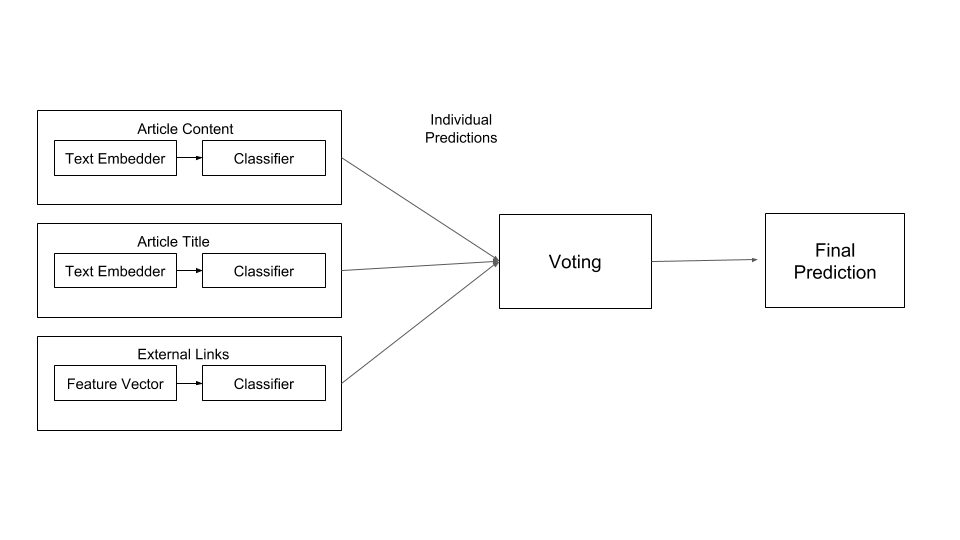
\includegraphics[width=8cm]{images/model.png}
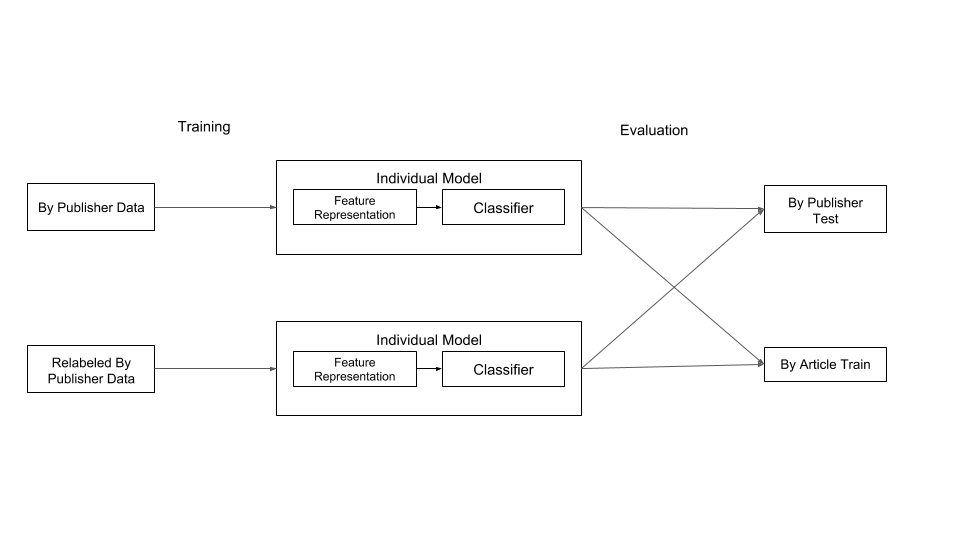
\includegraphics[width=8cm]{images/data_model.png}

\end{figure}

\section{Previous Work}

\textbf{Busagala et al., 2012} propose an ensemble of multiple types of automatic text classifiers which use various features \citep{6195332}. Similarly, we are incorporating various features into our model, so the results of this paper are useful to us. They experiment with linear SVM, polynomial SVM, and k-nearest-neighbors as their classifiers for their various features. For each feature they apply multiple classifiers and feed each classifier into a majority rule voting system. We experiment with majority voting as well as panel of experts. We use a single classifier for each feature type, instead of multiple classifiers.

\textbf{Bai et al., 2018} propose using sentence encoders for common NLP task instead of word encoders \citep{DBLP:journals/corr/abs-1803-01271}. They show that sentence embedders perform just as well as word embedders on many tasks such as sentiment analysis in movie reviews. They do this by embedding all the sentences in the text and then applying a Convolutional Neural Network (CNN) to the embedded representation. The sentence embedder which they propose is called the Univeral Sentence Encoder (USE). It is a Deep Averaging Network which averages the embeddings of all the words in the sentence, then feeds this average through a Dense Neural Network with 3 layers. Since the the articles are long we use sentence embedding to simplify the sequence modeling task. Instead of needing to classify based on hundreds of words in the article we can classify based on a few dozen sentences. We experiment with the USE and also use a CNN. 

\textbf{Cer et al., 2018} try to determine what architecture one should use for a given sequence modeling task \citep{DBLP:journals/corr/abs-1803-11175}. This paper informed our decision of what model to use to aggregate our sentence embeddings. We  use the simple Temporal Convolutional Neural Network (TCN) architecture they propose. The methodologies of this paper are to systematically discuss the benefits and drawbacks of various architectures for a range of tasks, and then to compare the results of those architectures. They show that TCNs outperform generic recurrent network architectures such as LSTMs and GRMs on a wide range of tasks such as copy memory and Penn Treebank character modeling. Additionally, the authors show that TCNs exhibit longer memory than RNNs with the same capacity. Like Cer et al., we use a TCN with dialated convolutions and residual connections. The architecture of this model is diagramed in Figure 2.

\begin{figure}[ht]
\caption{A) A dilated causal convolution with dilation factors d = 1, 2, 4. The receptive field is able to cover all values from the input sequence. B) TCN residual block. An 1x1 convolution is added when residual input and output have different dimensions. C) An example of residual connection in a TCN. The blue lines are filters in the residual function, and the green lines are identity mappings.}
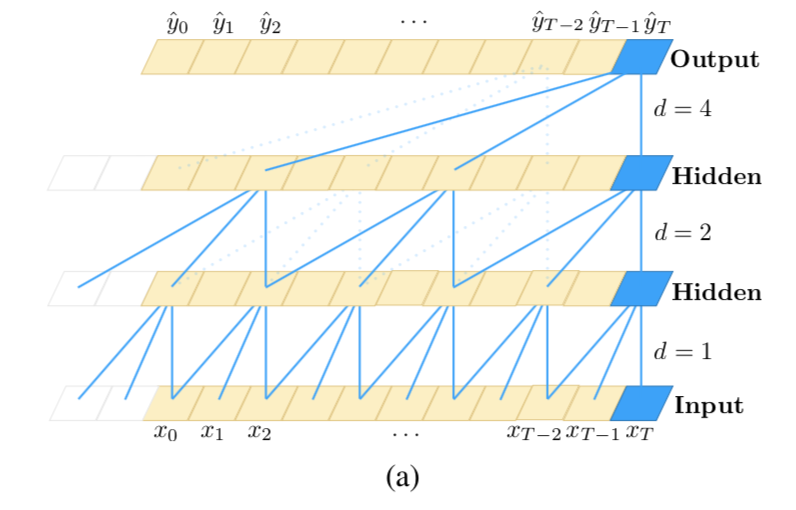
\includegraphics[width=8cm]{images/TCNN1.png}
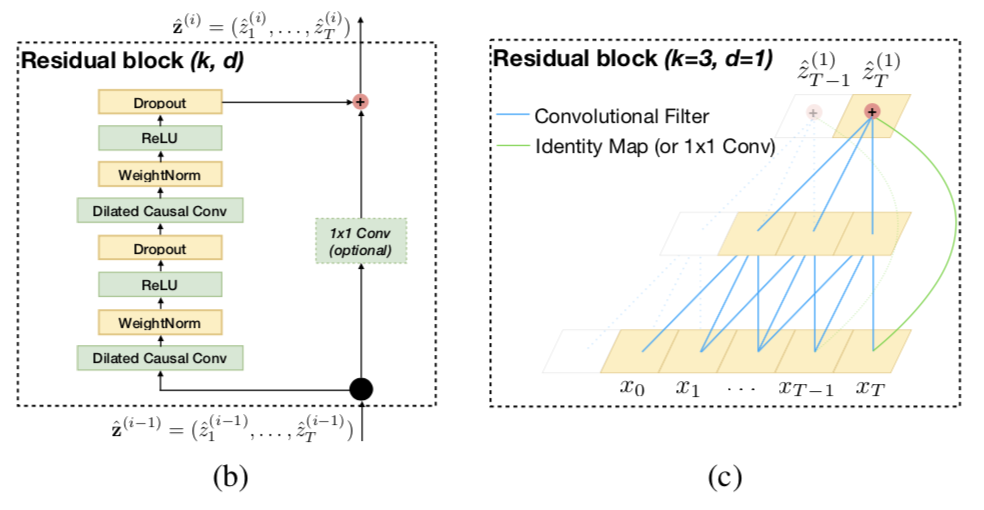
\includegraphics[width=8cm]{images/TCNN2.png}
\end{figure}

\section{Methodology}

Given a set of labeled news articles, we aim to build a model which can predict if a news article is hyper-partisan.

\subsection{Model}

Our model is composed of title, text, and links classifiers. The predictions from these classifiers are combined to generate a final prediction.

\textbf{Neural-Net Language Model:} To capture the semantic content of the title and text we used both word and sentence embeddings. The primary encoder we used was a Neural-Net Language Model (NNLM) trained on the Google 200B corpus \citep{Bengio:2003:NPL:944919.944966}. This was trained to simultaneously learn vector representations of words and predict the next word given the representations of the previous words. Given a word, the NNLM returned a 128-dimensional vector. We also used the NNLM to generate sentence embeddings by summing the word-vectors in the sentence and then dividing by the square root of the sum of the squares of the word-vectors. This naive method for combining words-vectors has been shown to perform well in practice.

\textbf{Universal Sentence Encoder:} We also tried a Universal Sentence Encoder (USE), which is a true sentence embedder \citep{DBLP:journals/corr/abs-1803-11175}. It uses a Deep Averaging Network to produce a 512-dimensional representation of a sentence. This was trained with a variety of data and Cer et al. reported very good transfer learning results. However, we found that the NNLM outperformed the USE. This may be because the NNLM was trained on news or because our model handles 128-dimensional vectors better than 512-dimensional vectors. In figure 3, a t-SNE of article title embedding clearly shows better separation with the NNLM. Since the NNLM did better than the USE, we used the NNLM for all of our experiments.

\begin{figure}[h]
\caption{Sentence embeddings of the article title. Hyper-partisan is dark blue and non-hyper-partisan is light blue. A) t-SNE of Neural-Net Language Model embedding. B) t-SNE of Universal Sentence Encoder embedding.}
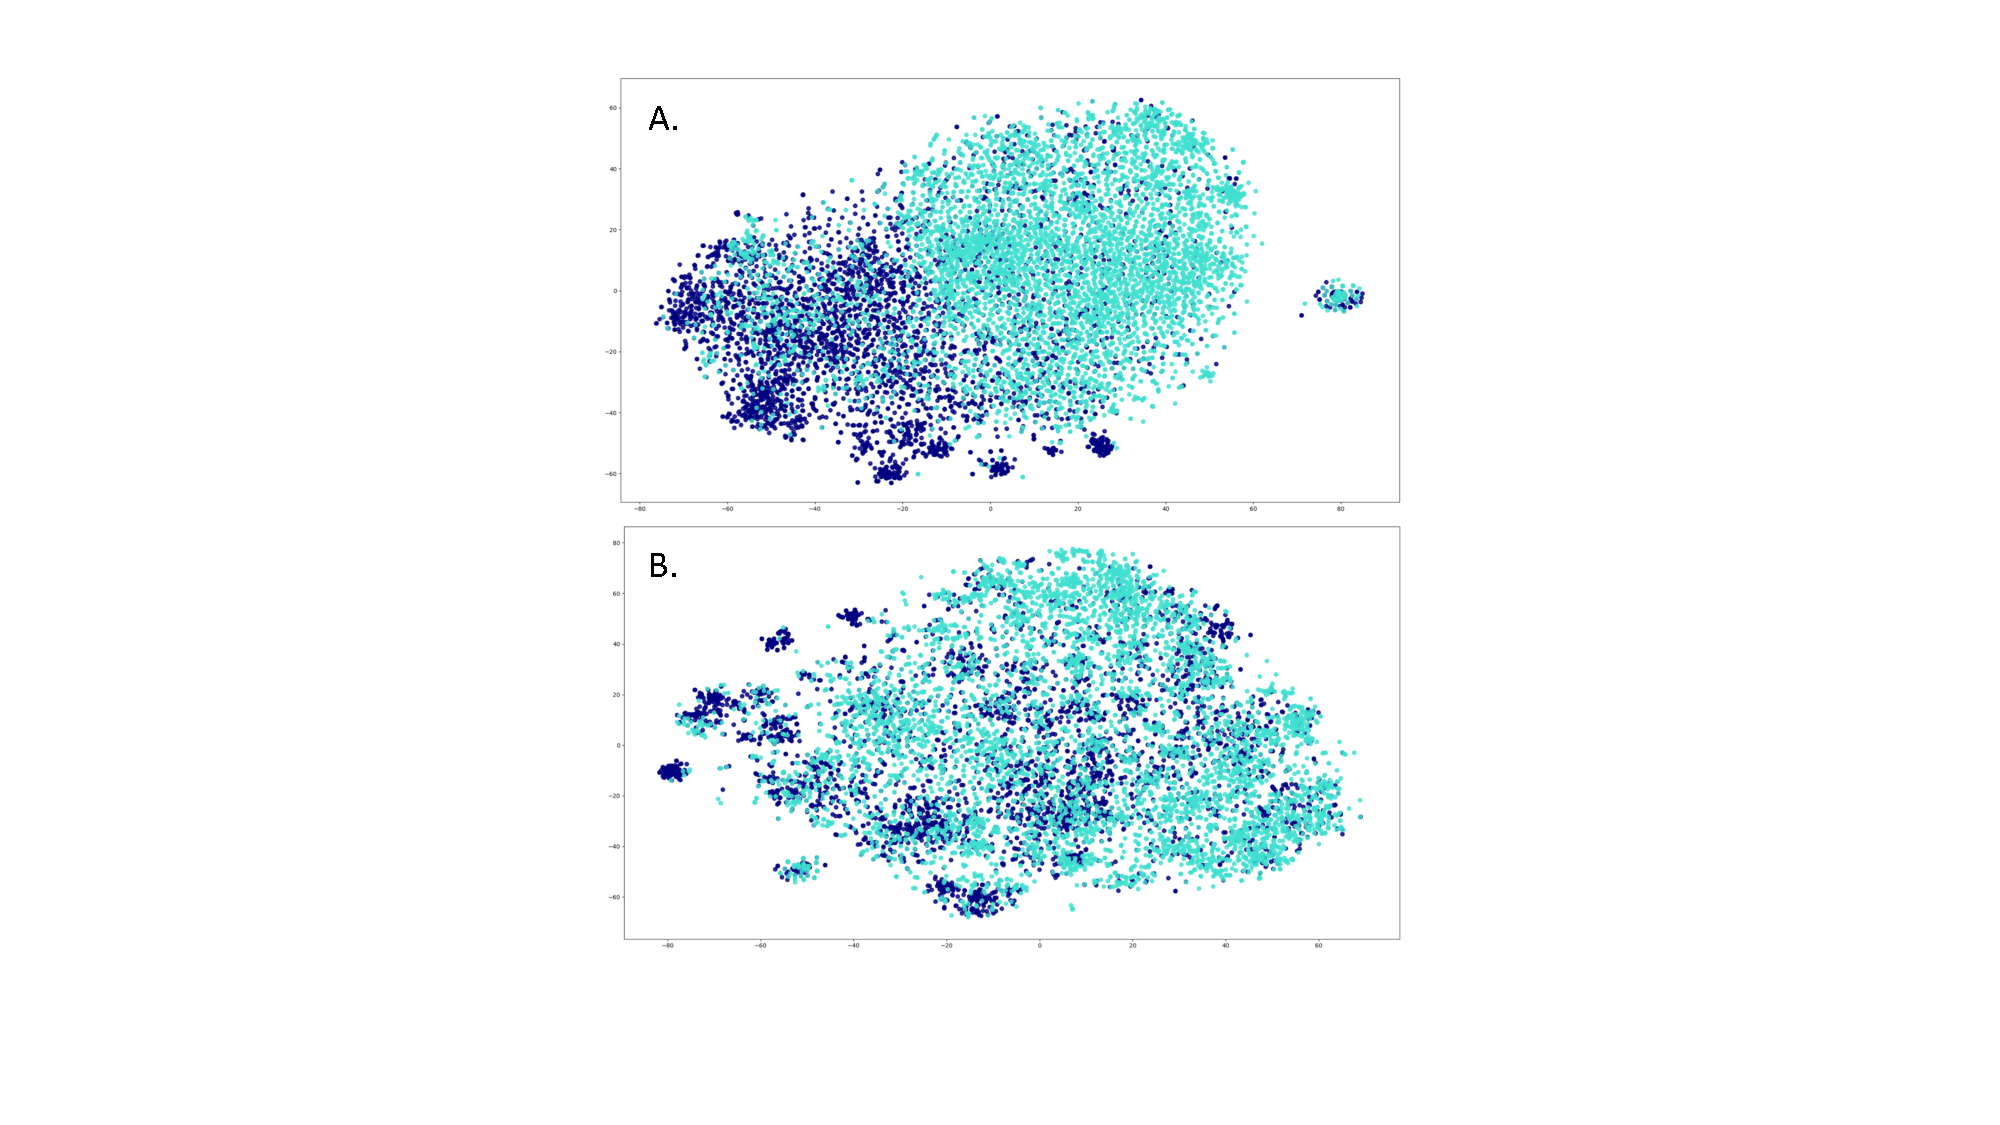
\includegraphics[width=8cm]{images/embedding.pdf}
\end{figure}

\textbf{Title Classifier:} To classify articles based on their title we used both word and sentence embeddings. For word embeddings, we encoded the first 32 words in the title. If there were less there were less than 32 words, we padded with empty strings. To aggregate the information from these 32 128-dimensional vectors we used a temporal convolutional neural network (TCN). This TCN had 128 filters, a kernel size of 2, and dilated by a factor of 2 from 1 to 32. We did not tune these hyper-parameters. For sentence embeddings, we encoded the articles title as a single sentence. This produced a single 128-dimensional vector for each article. To classify an article based on this vector, we used a dense nerual network (DNN). This 2-layer DNN had 256 neurons in the first layer and 56 neurons in the second layer. We choose this structure because the small number of neurons prevents over fitting. We selected a DNN over Naive Bayes because of the non-linear hypothesis space.

\textbf{Text Classifier:}  To classify articles based on their text we used both sentence embeddings. To do this we encoded the first 32 sentences and padded with empty string. We selected 32 because it is the mean number of sentences in the articles. Again we applied a TCN to the embedded representation. This TCN had 128 filters, a kernel size of 2, and dilated by a factor of 2 from 1 to 32. We did not tune hyper-parameters. We also tried embedding the first 256 words in the article and applying a TCN to this, but we found that is was too expensive in terms of computation and memory.

\textbf{Links Classifier:} To classify articles based on their external links we used a Naive Bayes classifier. We first created a domain vocabulary by extracting the domain for all the external links in the training data. This allowed use to generate a bag of domains feature vector for each article. We trained a Naive Bayes classifier using this bag of domains feature vector. We only considered the top 10,000 domains.

\textbf{Ensemble:} We created an ensemble with the best title, text, and links classifiers. We used two different voting mechanisms, majority voting and panel of experts, which is the normalized product of the probabilities given by the three classifiers.

\subsection{Data}

We trained and cross-validated our models on the 600,000 articles labeled by publisher provided by the Semeval challenge. We tested our ensemble on both the set of 100,000 test articles labelled by publisher and 600 articles from the hand-labelled training set.

\textbf{Relabeling:}
To alter the data with which we were provided and add to it more granular detail, we created a new, relabeled set of training data. Performing publisher-based cross-validation on the by-publisher training set, we relabeled each article for a given publisher with an ensemble trained on all other publishers in the set. Using the intuition that not all the publisher-based labels are inaccurate, this method normalizes our model's understanding of hyper-partisan-ness, ensuring it cannot get too skewed. The particular ensemble scheme we applied for relabeling was a Two of Three voting system. Of three models: a links classifier, a bag of words classifier, and a sentence-embedded title classifier using Naive Bayes, we relabelled if two of the three models were in agreement and over 80\% confident in their prediction. We selected these classifiers because they were easy to train and had simple hypothesis spaces which prevented over fitting.

\subsection{Training}

All models were trained with the same 500,000 examples from the v4 release of the Semeval hyper-partisan news data set. All TCNs and DNNs were trained for 10 epochs with cross entropy loss. Gradients were calculated with Atom (learning rate = .001) and 50\% of the neurons in each layer were dropped out to prevent over fitting. These defaults produced good results, so these hyper-perameters were not tuned. 

\subsection{Evaluation}

All models were evaluated on the v4 release of the semeval hyper-partisan news data set. We calculated accuracies for cross validation, test by-publisher, and test by-article. The cross validation set comprised of 100,000 examples from the training data which did not overlap with the 500,000 training examples. However, some publishers were represented in both the training and cross validation sets. When relabeling was used, both the training and cross validation sets were relabeled. The by-publisher test set contained 100,000 examples labeled by publisher and the by-article test set contained 600 examples labeled by article. These sets were never relabeled.

\subsection{Implementation}

Our models were implemented using scikit-learn and TensorFlow. Instead of writing low-level TensorFlow code, we used high-level APIs which make development faster. The text embedders were pre-built TensorFlow Hub modules. The USE can be downloaded from https://tfhub.dev/google/universal-sentence-encoder/2 and the NNLM can be downloaded from https://tfhub.dev/google/nnlm-en-dim128/1. We built our DNN using the high-level Keras API and used a pre-built Keras TCNN which can be downloaded from https://github.com/philipperemy/keras-tcn.

\section{Results}
\subsection{Model Performance}
We report a cross validation accuracy of 93\% on non-relabeled data, an accuracy of 66\% on the test data labeled by hand, and an accuracy of 60\%  on test data labeled by publishing organization. Our various ensembles performed best, with a panel of experts scheme resulting in the best cross validation results and a majority voting scheme yielding the best results on the hand-labeled data. We note that the top performing models were trained on data that had not been relabeled. Each ensemble relied on a combination of the Text Sentences, Title Sentences, and Links, models. Results for each model and ensemble can be seen in figure 4. 
\begin{figure}[ht!]
\caption{Here we compare results for our individual models, trained on both data that has not been relabeled and data that has been relabeled with a Two of Three Agree scheme, and our best performing ensemble, trained on the same two sets. The three graphs depict accuracy for cross validation, data labeled by-publisher, and hand labeled data. Each ensemble relied on a combination of the Text Sentences, Title Sentences, and Links, models.}
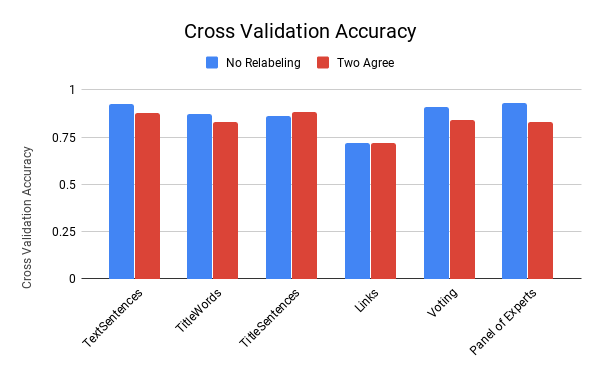
\includegraphics[width=8cm]{images/models_cross_val.png}
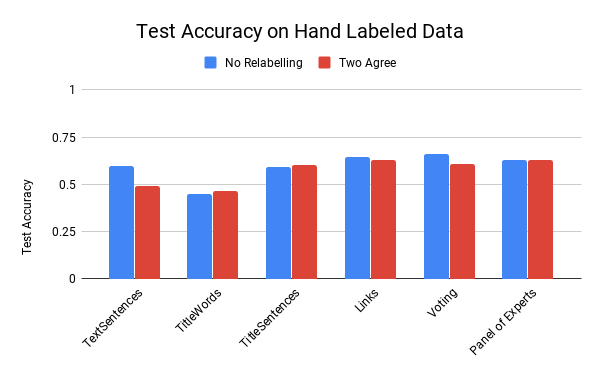
\includegraphics[width=8cm]{images/models_by_hand.png}
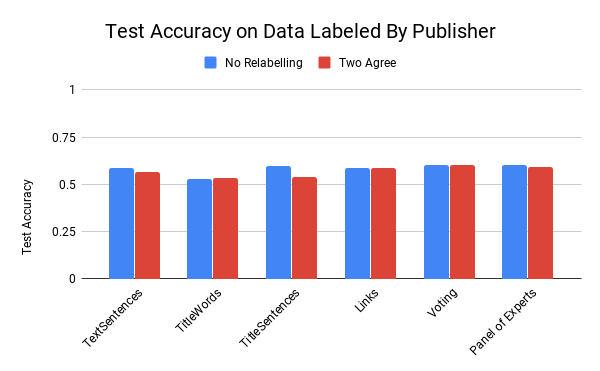
\includegraphics[width=8cm]{images/models_by_pub.png} 
\end{figure}
\subsection{Relabeling}
Though our model performed better in most instances without relying on relabeled data, we are encouraged by this method of relabeling. Figure 5 depicts the most frequently relabeled publishers. Despite the conclusions one would draw from first glancing at the URLs, a further look into the publishers indicates that our model is performing well at correcting aberrant labels. Take, for example, the publisher most often relabeled as hyper-partisan. Though the name Foreign Policy Journal sounds innocuous, much of its content has a discernibly hyper-partisan bent. Conversely, though The Washington Times caters towards conservatives, contrary to the labeler's decision, many of its articles stay close to neutral. 

\begin{figure}[ht!]
\caption{A graph of the publishing organizations whose articles were most often relabeled by our Two of Three voting system. The values represent the percentage of each organizations articles that were relabelled. The first figure is the publications that were initially labeled as not hyper-partisan that our scheme relabelled as hyper-partisan and the second is the reverse.}
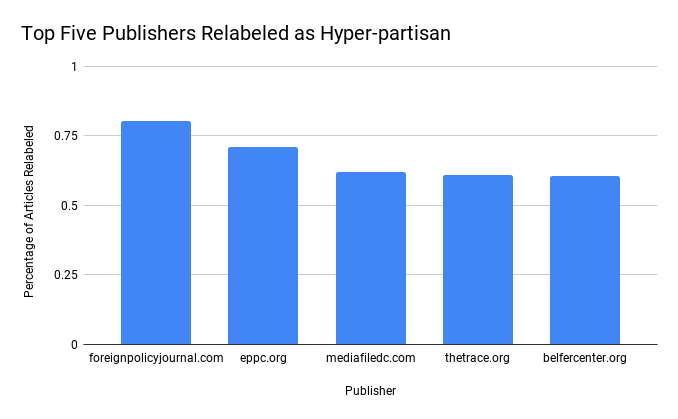
\includegraphics[width=8cm]{images/relabel_hyp.png}
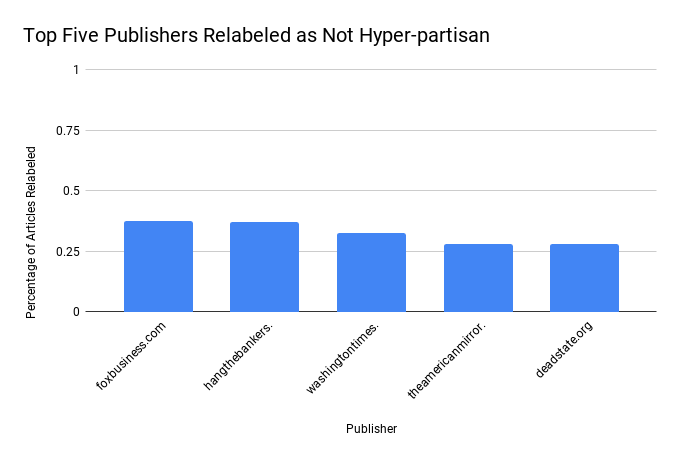
\includegraphics[width=8cm]{images/relabel_not_hyp.png}
\end{figure}


\section{Discussion}

\subsection{Model Performance}
We show that a combination of simple feature representations (in the form of article links) and deep learning techniques performs well on the task of hyper-partisan news detection. A temporal convolution network that runs on top of sentence embeddings of article text yields 92\% cross validation accuracy. While our model's test accuracy is fairly low, we chalk this up to the lack of granularity of labeling in the training data and the by-publisher evaluation data. We also note our model's noticable improvement on a simple bag of words classifier on the same set. We achieve a 60\% evaluation accuracy on test data that has been labeled by publisher, but note the innaccuracies in the labeling set. Vox news, for example, despite its left-leaning bent is not hyper-partisan. A better gauge of our model's performance is the 66\% accuracy it gets when evaluated on hand-labelled data. This score is 6\% increase from the by-publisher set, but that in part can be ascribed to this set having many overlapping publishers with our training data. The low performance again may have to do with a the distorted training data. Though we implemented a relabeling mechanism that was ultimately unsuccessful in yielding higher accuracy, we note that we were relabeling bad data with other bad data. A more nuanced approach to this problem, and a future direction for our project in advance of the Semeval competition, is to iteratively relabel the set, perhaps also by hand curating which publishers are excluded from the training of the relabeler. Additionally, leveraging the probability distributions per publisher of the hand labeled training data may yield a more nuanced relabeling of the larger training set.

\subsection{Performance by Publisher}
When comparing our different models, one aspect of note that arises is their differing strengths. The links-based models perform well on different publishing organizations than the models that rely on textual elements of an article perform well on. See figure 6 for a breakdown of the differences. This is an encouraging avenue for further research, for we can pursue an ensemble strategy that intuits each model's strengths and leverages them. 
\begin{figure}[ht]
\caption{This graph depicts the differing strengths of a text based model and a links based model. Aggregating the by publisher results from the models that relied on the body text or title of the article, we sorted by the top performing publishers in this category, averaged all whose accuracy scores were above a 90\% threshold and graphed it against the corresponding average for the links based model. When sorting by links, we did the same, but with a more generous threshold of 80\%.}
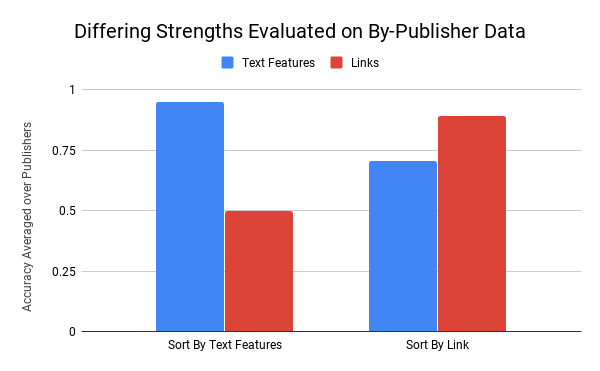
\includegraphics[width=8cm]{images/links_vs_article_by_pub.png}
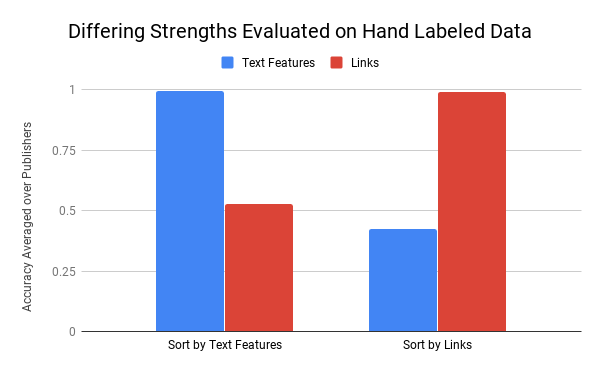
\includegraphics[width=8cm]{images/links_vs_article_by_hand.png}
\end{figure}

\section*{Acknowledgments}

We would like to thank Rich Wicentowski for his guidance on this project.

\bibliography{naaclhlt2019}
\bibliographystyle{acl_natbib}

\end{document}
